\section{ SR0020BE10 }


\subsection{Meta}

    \textbf{Title:}
    Operating room planning and scheduling: A literature review

    \begin{table}[H]
        \centering
        \begin{tabular}{|c|c|c|c|c|c|c|c|c|}
            \hline
                \textbf{Rank} & \textbf{Grasp} & \textbf{Grade} & \textbf{Type} & \textbf{Outcome} & \textbf{Domain} & \textbf{COV19} & \textbf{CoI} & \textbf{DB} \\
            \hline
                4 & 96\% & A & A & P & S & No & ?? & No \\
            \hline
        \end{tabular}
        \caption{Reference's metadata}
        \label{tab:SR0020BE10}
    \end{table}

\subsection{Summary}
    Brecht Cardoen, Erik Demeulemeester, and Jeroen Beliën \cite{x228} produced an easy-to-follow literature review regarding operating room planning and scheduling. The review contains all the most crucial aspects of OR planning and scheduling in a structured, coherent form. The authors analysed the reviewed studies by patient characteristics, performance measures, decision levels, research analysis types, solution techniques, uncertainty, and application of research. The lack of practical solutions is highlighted, and examples of the most common obstacles are described in detail. This literature review can be considered the most user-friendly paper for beginners in medical resource planning and scheduling.

\subsection{Notes}
    \begin{itemize}
        \item DBs: Pubmed, Web of Science, Current Contents Connect, Inspec;
        \item Data envelopment analysis (DEA);
        \item Garey and Johnson (55) - problem complexities;
        \item Implemented (10, 12, 13, 14, 53, 64, 109);
    \end{itemize}


\subsection{Reading}
    \textbf{Abstract:}
    This is a literature review on the publications resent in 2010. The problem formulation and solution development aspects was considered in the reviewed literature.
    
    \textbf{Objectives:}
    The aim is to summarise the current trends in operating room planning and scheduling, and identify the directions for further research.
    
    \textbf{Page 1-3 (Introduction):}
    The importance of the operating rooms in the healthcare management system in hihglighted in the introduction of this literature review. The authors give general information on the history of the research in the overviewing field, outline the structure of the review, mentioned some boundaries, datasets used in the research, and note the increased interest in the field from 2000 to 2010 in comparison with timespan 1950-1999. 
    \begin{figure}[H]
        \centering
        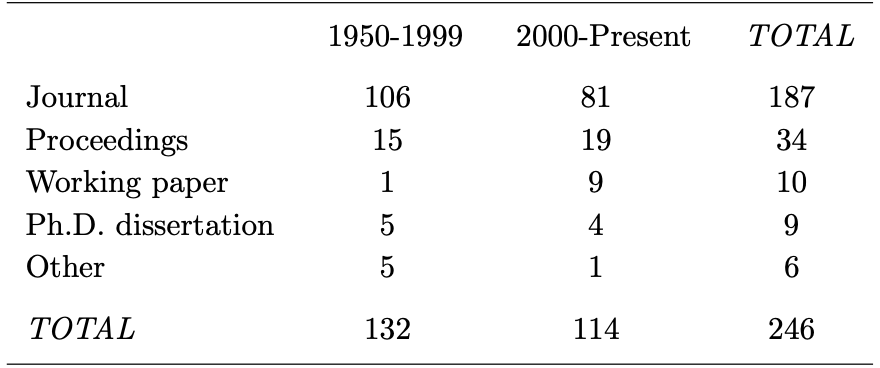
\includegraphics[width=1\textwidth]{figures/SR0020BE10/fig1.png}
        \caption{Distribution of the reviewed papers by years of publication from \cite{x228}.}
        \label{fig1:SR0020BE10}
    \end{figure}
    
    \textbf{Page 4-5 (Organisation of the paper):}
    The authors undeline seven fields of analysis: patient characteristics, performance measures, decision level, type of analysis, solution technique, uncertainty, applicability of research. During introduction of each of the fields, the authors will try to categorise the liteeatre according to these fields.

    \textbf{Page 6-7 (Patient characteristics):} 
    Elective or Non-elective, inpatients or outpatients. Non-elective has also urgent or emergent patients (reflection: classical classification as for now, but maybe not in 2010). There is a paper which proves that if the reserved capacity for non-elective patients is spread amoung various operating rooms, the overtime and the overall operating room utilization significantly improves.
    
    \textbf{Page 7-11 (Performance measures):}
    Introduction and examples in literature of the next metrics: waiting time, opearting room idle time (surgeon idle time), overtime, stakeholders fulfillment.
    
    \textbf{Page 11-14 (Decision level):}
    The authors outline four decision levels: discipline, surgeon, patient, and other. The planning and scheduling solutions are designed in respect of surgery date, time, room, capacity and other metrics. The downstream capacities are closely interconnected with the operating theatres, therefore optimise the surgery scheduling ignoring ICUs or PACUs can lied to reducing in efficiency of the scheduler.Nevertheless, more than half of papers research the scheduling approaches with the opearting rooms in isolations from other capacities.  
    
    \textbf{Page 15-19 (Type of analysis):}
    For the operating theatre planning an scheduling the scenario analysis most oftenly used. Here the literature hard constraints have been described with examples found in literature. 

    \textbf{Page 19-23 (Solution technique):}
    Column generation approach allows to start with essential hard constraints and after some simple solution is found introduce more complexiti into model by adding new soft constraints. This section hihglights some of the existing computer methods for OR planning and scheduling. There is even work with an analytical approach.

    \textbf{Page 23-25 (Uncertainty):}
    Uncertainty is a notable obsticle in the OR planning and scheduling whihc for the most times is managed with simulation, stochastic, or both models.
    
    \textbf{Page 25-26 (Application of research):}
    By 2010 there is almost no practical implementations for the planning ans scheduling approaches in real envirnments.
    
    \textbf{Page 27 (Conclusion):}
    The most valuable hihglights from the conclusion: (1) simulation and scenario analysis are most common techniques to understend and address the OR scheduling problem; (2) Most OR are scheduled in isolation, but more practical method is to include up- and downstream capacities too; (3) The gep between model development and practical implementations should be addressed in the future research. 